\documentclass{article}
\usepackage[utf8]{inputenc}
\usepackage{graphicx}
\usepackage{float}

\usepackage[sorting=none]{biblatex}
\addbibresource{references.bib}

\title{Tracking everyday sleep \\ Final Report}
\author{Emil Ståhl, Ronas Baran, Hector Gonzalez Campos}
\date{February 2021}

\begin{document}

\maketitle

\section{Introduction}
This chapter gives an introduction to the project.

\subsection{Background}
It is said that we on average spend about a third of our life sleeping.  A good night's sleep is vital for every human being to survive and function properly. Experimental research has clearly shown the negative impacts of sleep deprivation.\cite{ohlmann_costs_2009} However, there is none to little research showing how the variations in our sleep that arise in our daily life affects well-being and general performance. Therefore, Stockholm University (SU) is performing a study called “Sömn i vardagen” (everyday sleep) where they are going to study how length and quality of the sleep changes on a day to day basis as well as if there is a difference between young and older people. This will then be used to study how it affects mood and performance of the users participating.\cite{schwarz_anslag_nodate}

\subsection{Purpose}
The purpose of this report is to extend our knowledge about developing mobile applications, its requirements and what is key for achieving a good user experience. This will be achieved by working on a real-world mobile application with clear specifications from the client. 

\subsection{Goal}
The goal of this project is split into two different areas, the first part of the goal is to learn the techniques used for developing mobile applications as well as how to design an application in order to maximize the user experience. In addition to this, these goals will be achieved by developing an application that is going to be used as an inspiration for the actual application used in the official study at SU. The researchers in the area can then use the data collected by the app in order to study user behaviour and draw meaningful conclusions that hopefully leads to a better understanding of the problem. Two different techniques will be used for developing two different working prototypes, these techniques are JQuery for developing an web application, additionally, an native application will be developed for the Android platform. 

\subsection{Benefits, ethics and sustainability}
There are many possible benefits that may result from developing an application that can track a user's sleep and health. The United Nations has established 17 goals for sustainable development (SDG), one of which includes good health and well-being. By developing this application it can potentially lead to a more sustainable world since good health has direct impacts on other SDGs leading to a positive long term effect. While there are many areas of application that can be of benefit to society, there are also ways to abuse the technology. In a dystopian society, sleep tracking is used to control and surveil the people. This would be a grave infringement on the personal integrity of the people and could contribute to the power of a totalitarian government. Despite this potential abuse of the technology, contributing to the common person’s understanding of sleep tracking can decrease the room for abuse, as people realize the power of the technology and consequently actively resist its abuse. An aspect of sustainability exists when considering the development and usage of sleep tracking systems. All forms of digitization inevitably lead to further dependency on electricity.\cite{noauthor_17_nodate}

\subsection{Methodology}
In this report, the method consists of a field study researching the general public’s view on sleep tracking, this will then be used to develop a paper prototype that will be used for gathering user feedback that will be considered while developing the functional prototypes. 

\subsection{Outline}
In this report, there are 3 chapters.
Chapter one is an introduction to the thesis where the background is briefly explained and what problem will be researched and examined. Shortly the purpose, the goal, and the method are explained and also what connection it has to ethics and sustainability. Chapter two explains the design process including a field study and the development of the paper prototype, web app prototype and Android Prototype. Chapter three contains discussions of the application’s impact on the market as well as an analysis of the design choices. 

\section{Design Process}
This chapter covers the development of the paper prototype, the field study and the development of the two mobile applications.

\subsection{Paper Prototype}
A low-fidelity paper prototype was created using Figma, shown in Fig. 1. The main screen of the prototype shows surveys represented as cards that the user has to complete, clicking on one of the surveys will enlarge it so the user can answer.  The settings page will allow the user to set up and change their sleep schedule. The profile page will allow the user to see their profile and potentially statistics regarding their sleeping habit.  Lastly, there is an information page where the user will be notified about vital information regarding the research study and the application.
 
For doing our design we based on the principles design where we consider to have white space, align the elements among them, similar colors in objects with the same functionality like buttons, paragraphs.\cite{galitz_essential_2007} Moreover,  we use the proximity between elements that are related to form groups that are visually easy to identify.

\begin{figure}[!h]
  \begin{center}
    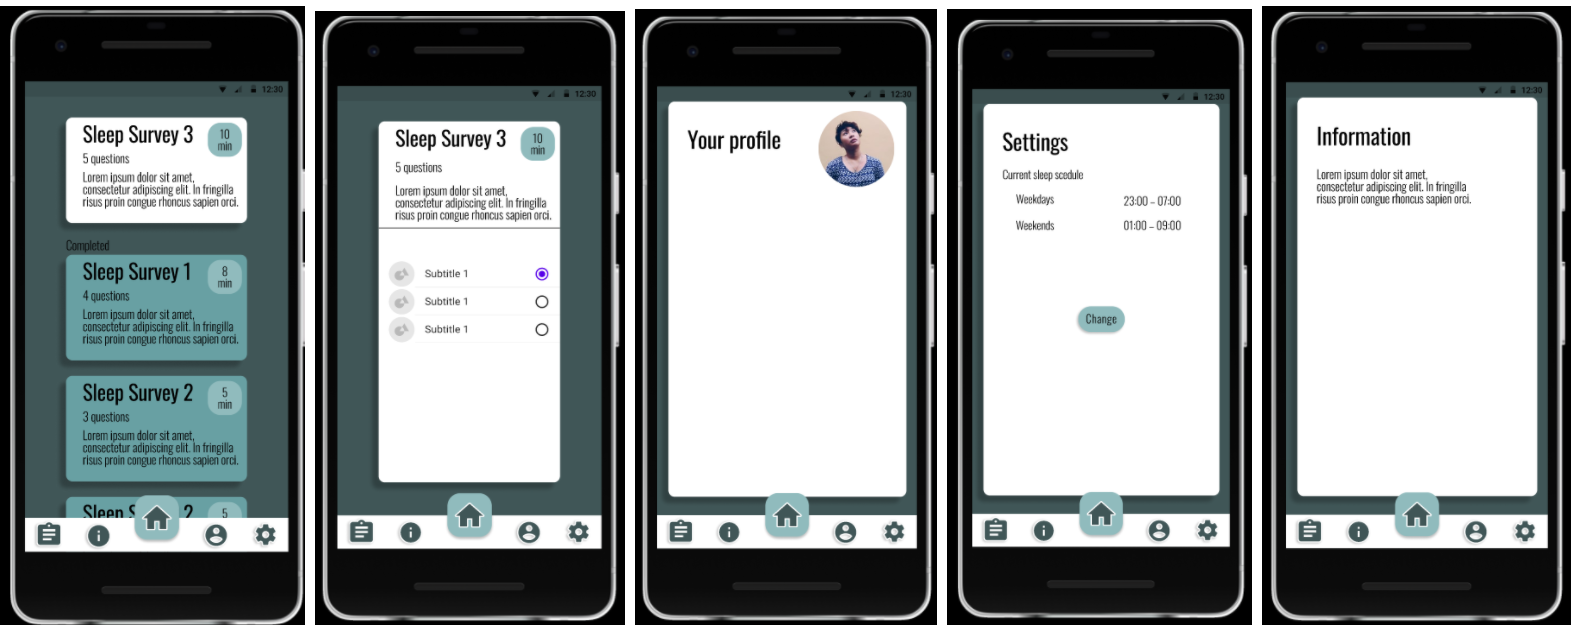
\includegraphics[scale=0.8]{FigmaPrototype.png}
    \caption{The different pages in the prototype}
    \label{fig:figmaPrototype}
  \end{center}
\end{figure}

\subsection{Field Study}
This chapter explains the field study, how it was performed and its results. 

\subsubsection{Survey}

Since the chosen topic for this project was pre-determined by the research project, we chose to focus our field study on firstly, people’s motivation for using sleep tracking apps and secondly, the usability and design of our prototype. For the first part we asked questions concerning their previous usage of sleep tracking apps and their attitude towards them. The outcome of this will have an effect on how we chose to design our application. If people in general have a bad attitude towards these kinds of applications, we might have to design and implement more functionality to make the users keep using our application. However, if their attitude is good, they might come back even with the basic functionality. We also added a question about people’s attitude towards joining a research project by using a sleep tracking application, for the same reason. 

The other part of the survey was more focused on the design of our prototype. We asked the participants to perform a simple task in the prototype, namely to change their wake up time and then rate the difficulty from 1-5, low numbers being easy and high numbers being difficult. They were also asked to rate the overall design from 1-5, where the higher the number represented how enjoyable they thought it was. Since our application will be used by a wide variety of ages it is important that it is simple to use by all ages. 

\subsubsection{Results of field study}
The following section is a summary of our results from the survey. There were 18 answers in total and the largest age group were 18-29 (11 people). The other age groups that were represented in the answers were 30-39 (4 people), 65+ (2 people) and 40-49 (1 person). 

The diagram below shows the answers to the first question about sleep tracking applications, seen in Fig. 2. There was an introduction and our definition of Sleep tracking application provided in this question. 

\begin{figure}[!h]
  \begin{center}
    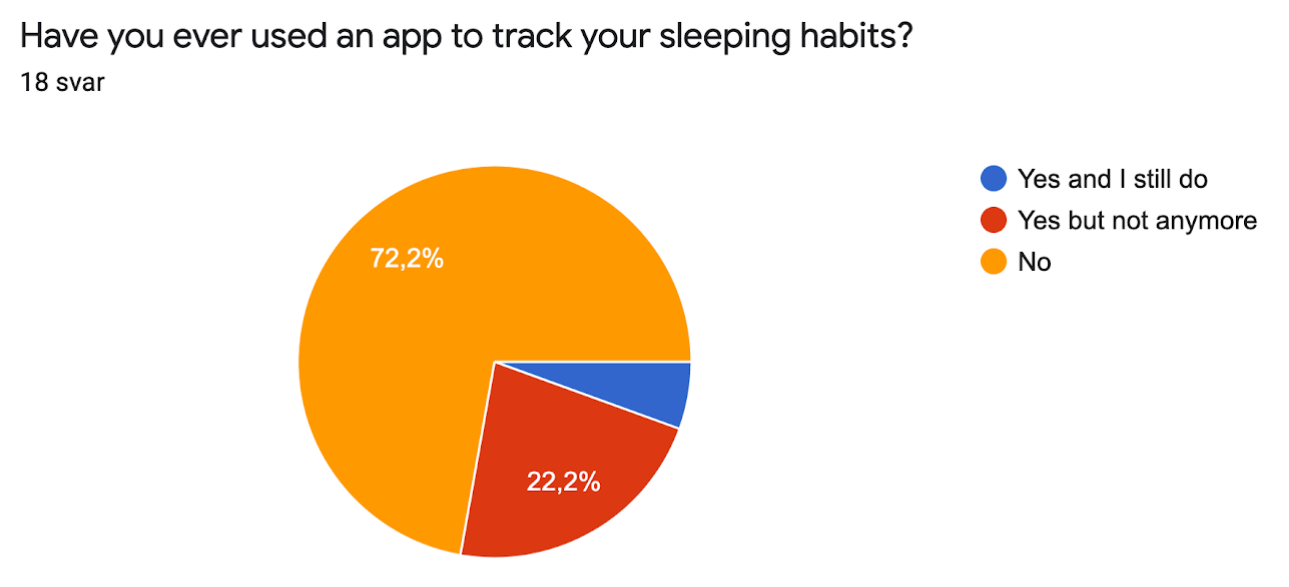
\includegraphics[scale=0.8]{Diagram1.png}
    \caption{Answers to first question about sleep tracking applications
}
    \label{fig:diagram1}
  \end{center}
\end{figure}

A majority of the persons answering this survey had never used a sleep tracking application. A more interesting result is that out of the 5 persons that had used these apps, 4 of them had stopped. The four people giving this answer were spread out over the age groups. …..This might be indicating that the apps available on the market today, are having a hard time keeping their users. The next question was directed to those people that have answered that they had stopped using these apps, asking them to write the reason why they stopped. We got the following answers:

“I did not think it helped me”
“Did not feel like it gave me anything”
“I am very forgetful and did not remember to use it and it was not very intuitive to use”
“Stressed me”

The two first answers concerns if the app is fulfilling its purpose for the user, which in these cases they did not feel like it did. They felt that the app did not help and give them anything. 

For the third question, we wanted to look into their attitudes towards using a sleep tracking app for research purposes. The majority of the people we asked answered that they would be willing to participate in such study, only three answered that they would not. An interesting result is that everyone that stopped using these apps answered that they would be willing to participate. 

The following graph displays the outcome of our questions about the design, see Fig. 3 and 4. 

\begin{figure}[!h]
  \begin{center}
    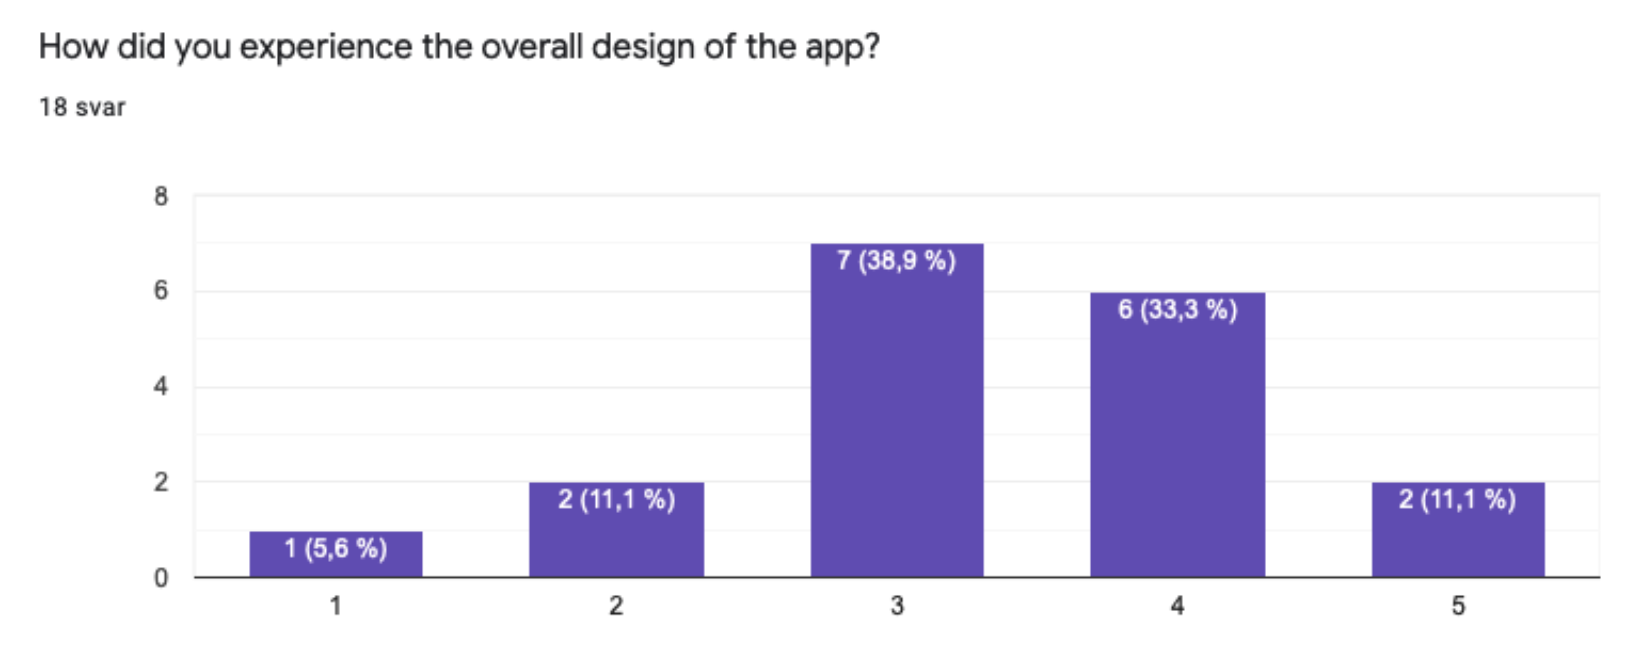
\includegraphics[scale=0.6]{Diagram2.png}
    \caption{1 represents terrible and 5 represents perfect.
}
    \label{fig:diagram2}
  \end{center}
\end{figure}

What is interesting is that the average experience of the design was lower for people over 30 than under 30 with an average of 2.85/5 compared to 3.63/5. This might suggest that the current design is somewhat more catered towards the younger demographics which is something that needs to be considered and looked into since the application will be used by other demographics as well. 
\begin{figure}[!h]
  \begin{center}
    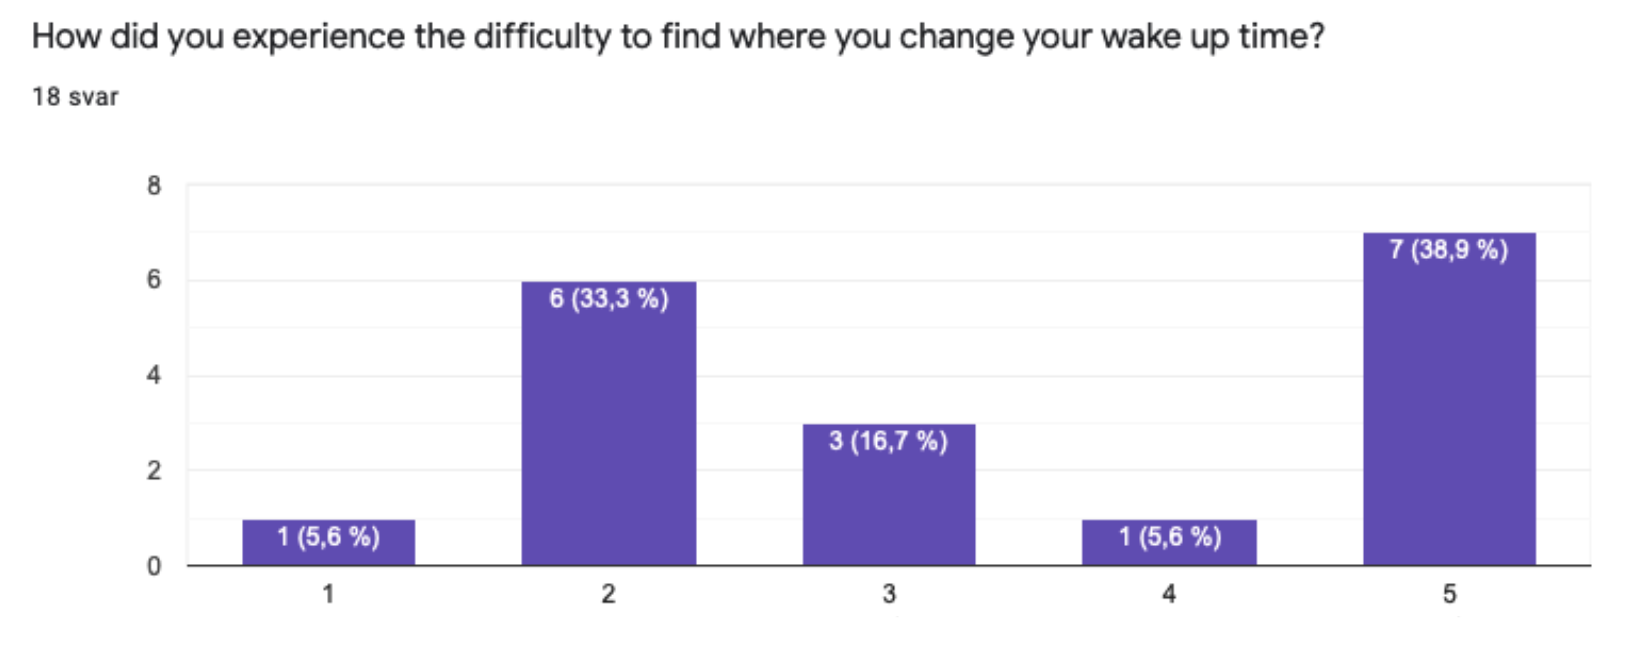
\includegraphics[scale=0.6]{Diagram3.png}
    \caption{1 represents terrible and 5 represents perfect.
}
    \label{fig:diagram3}
  \end{center}
\end{figure}

The results were pretty similar regarding the difficulty when navigating. However, it is important to mention that after the answers had come in it came to our attention that the prototype did not work for iPhone users, making these results unreliable.

\subsection{Web App Prototype}
For developing the first prototype we chose to do a web app utilizing the Javascript library called JQuery Mobile. This simplifies HTML DOM tree traversal and manipulation as well as CSS animation. The reason for using jQuery is that it takes a lot of common tasks that require many lines of JavaScript code to accomplish, and wraps them into methods that you can call with a single line of code.

\subsubsection{Implementation}
When we implemented the web app prototype we chose to follow our previously created paper prototype developed with Figma. We chose this design because the user feedback showed both positive and negative things about both versions and it was a unanimous decision by the group that this was the best way forward, however the user feedback was taken into consideration. We are focusing on making the app as easy to use as possible and we feel that our chosen prototype could make  that possible. 

Figure 5 shows the final design and implementation of our Figma prototype as a web app. We tried to follow the design as much as possible but we soon found it is difficult to work with tools that we were not very experienced in. In figure 6 we can see that clicking on one of the surveys opens up a popup screen for the user.

\begin{figure}[!h]
  \begin{center}
    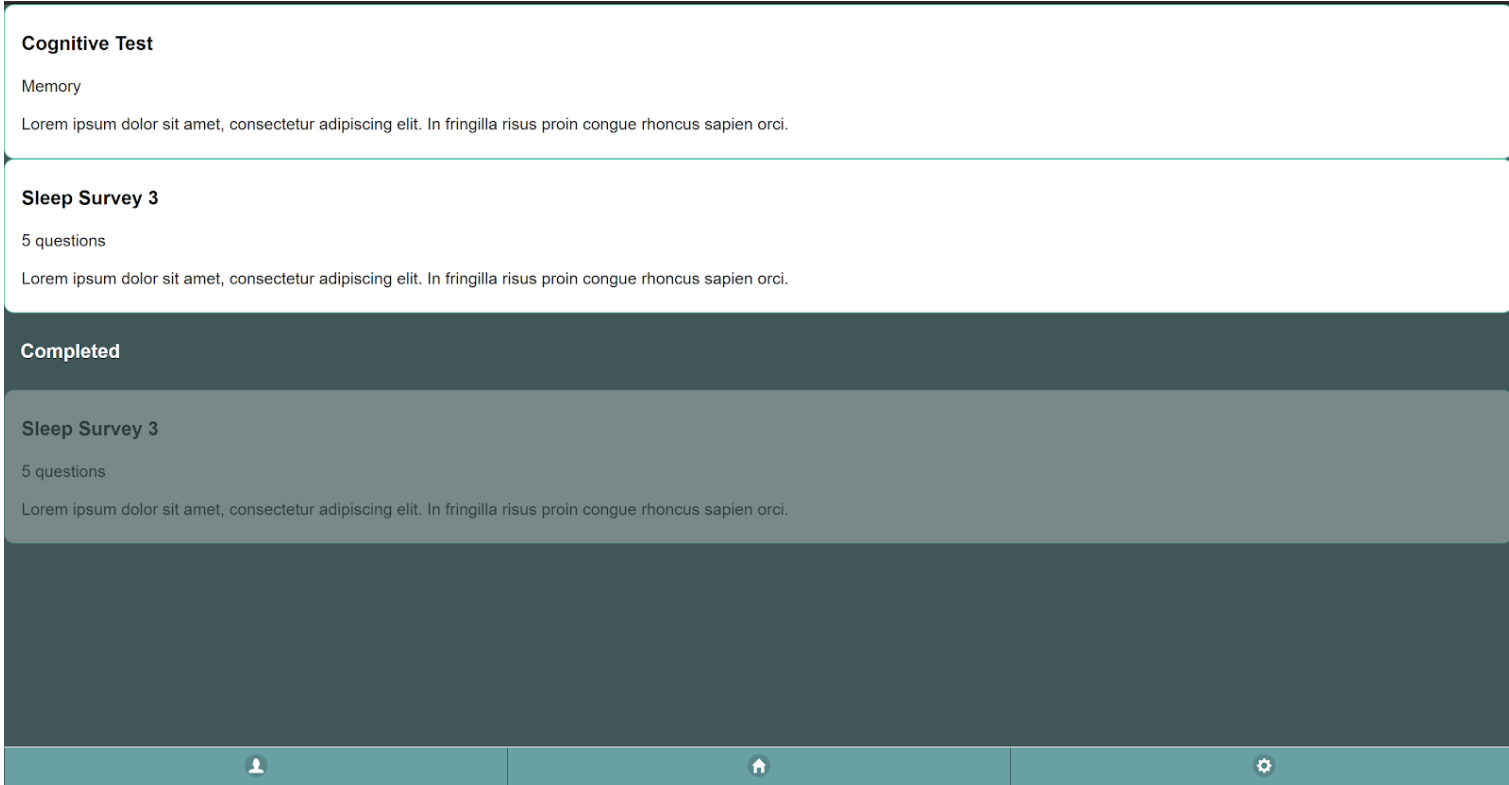
\includegraphics[scale=0.8]{WebApp1.png}
    \caption{The popup when clicking on Sleep Survey 3
}
    \label{fig:webapp2}
  \end{center}
\end{figure}

\begin{figure}[!h]
  \begin{center}
    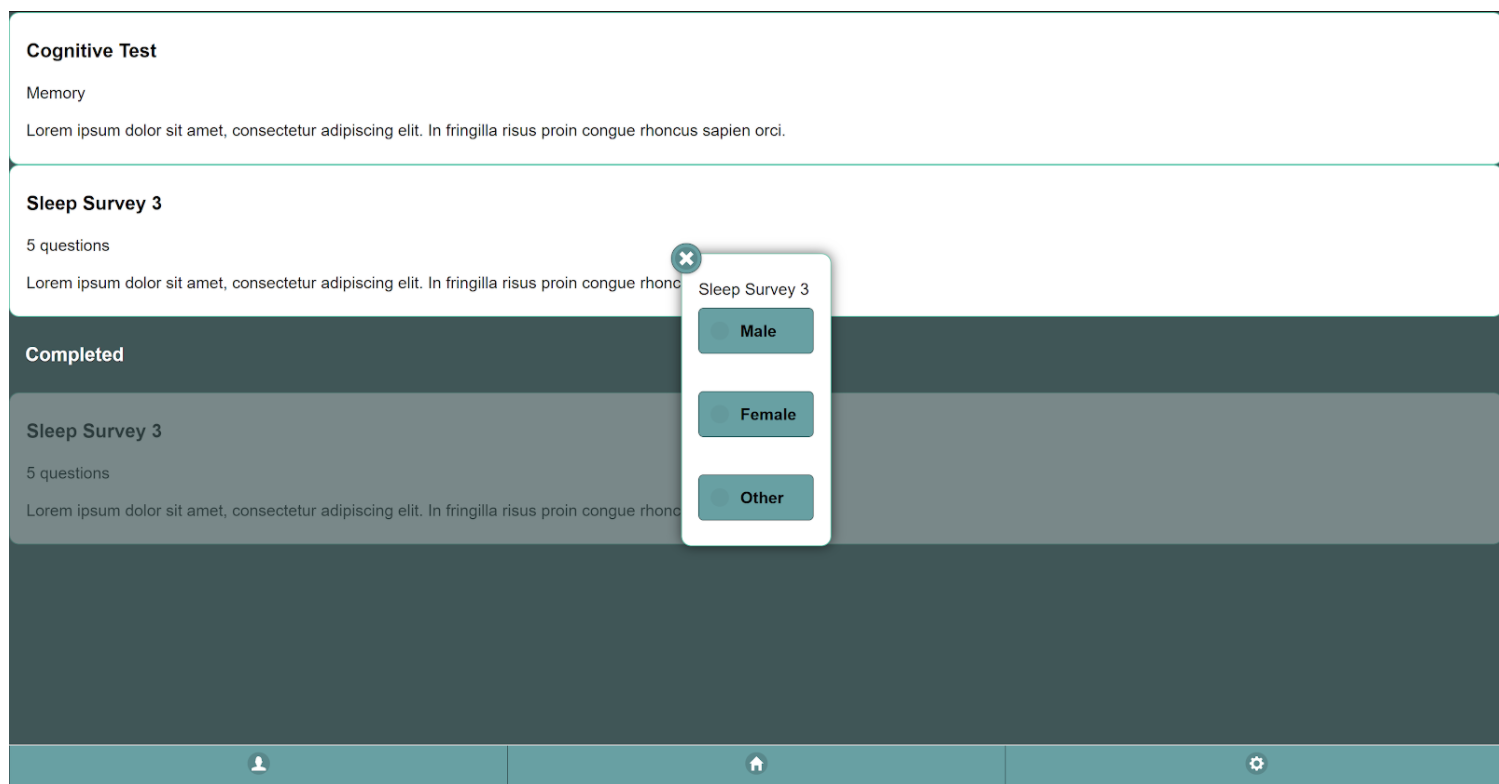
\includegraphics[scale=0.8]{WebApp2.png}
    \caption{The main screen of the web app
}
    \label{fig:webapp1}
  \end{center}
\end{figure}

The navbar that can be seen at the bottom of the page in Fig. 5 and 6 was implemented in HTML with the following structure: 

\begin{verbatim}
           <div data-role="footer" data-position="fixed" class="ui-footer">         
       	<div data-role="navbar" class="ui-navbar" >
            	<ul>
                  	<li><a href="a" data-icon="user"></a></li>
                        <li><a href="a" data-icon="home"></a></li>
                        <li><a href="a" data-icon="gear"></a></li>
            	</ul>
       	</div>
       </div>
\end{verbatim}
Jquery Mobile will identify the data role in a DOM element and apply the characteristics of that specific data role, in our case it is the footer, and inside it, we add the navigation bar.

The different tests and surveys were implemented as simple div tags: 

\begin{verbatim}
    
         <div class="ui-body ui-body-a ui-corner-all">   
             <H3>Cognitive Test</H3>
             <div  >
             	<p>Memory</p>
             	<p>Lorem ipsum dolor sit amet, 
             	 consectetur adipiscing elit. In fringilla 
             	 risus proin congue rhoncus sapien orci.</p>
     		 </div>       
      </div>
\end{verbatim}

\subsection{Android Prototype}
The Android prototype was implemented using the Android Studio IDE in the Kotlin programming language. The implementation of the prototype was divided into two parts that were developed sequentially. The first part, that internally was referred to as the “main” phase”, concerned the development of the bottom navigation menu and the four pages that the menu leads to. The second part was referred to as the “task” phase and concerned the task that was assigned to the group regarding the research project. 

\subsubsection{Main Phase}
During the development of the “main” phase results from the user feedback indicated that the applications UI design was lacking and could use some extra work. Referring to the design guidelines of Google’s Material Design was therefore very helpful.\cite{noauthor_material_nodate} This can be noticed when comparing the Android prototype with the Figma prototype, where the menu for the latter was deemed to be confusing according to user feedback. As a consequence the central home button was removed and a more minimalistic style menu was implemented. To further follow the guidelines, one area of improvement would be to remove the settings from the bottom navigation bar and instead have it be accessed from the profile page.

\subsubsection{Home Screen}
The app’s home screen consists of a navigation bar along with cards that represents the different cognitive tests and questionnaires. Clicking on the cards will take the user to the respective screen. The reasoning behind the use of cards was to give a compact and clean look while also being easy to understand.

\begin{figure}[H]
  \begin{center}
    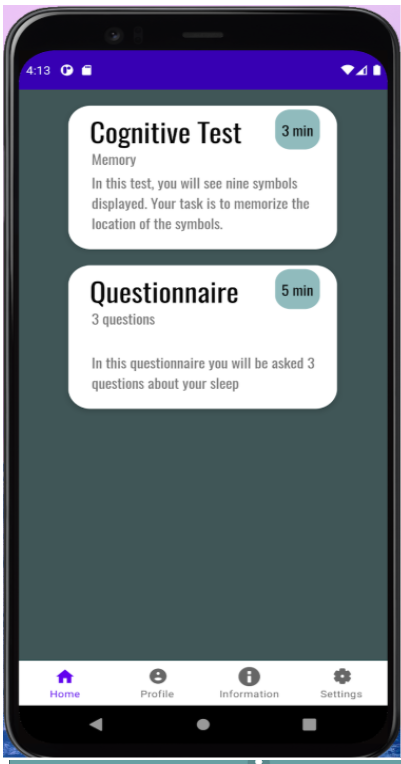
\includegraphics[scale=0.8]{Android1.png}
    \caption{The home screen of the app
}
    \label{fig:android1}
  \end{center}
\end{figure}

\subsubsection{Settings}
The settings page lets the user adjust the wake up time and bedtime, i.e. when the app should notify the user about doing the questionnaire. Here, the user can also enter its contact information.

\begin{figure}[!h]
  \begin{center}
    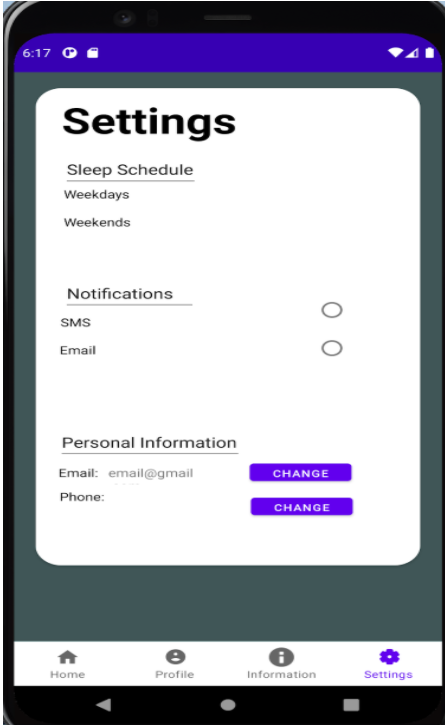
\includegraphics[scale=0.8]{Android2.png}
    \caption{The settings screen of the app
}
    \label{fig:android2}
  \end{center}
\end{figure}

\subsubsection{Profile and Information}
The last two parts are profile and information where the user can see its user id and contact information. The information page gives info about the app and the study. Future work could focus on displaying the user’s statistics on the profile page. 

\begin{figure}[!h]
  \begin{center}
    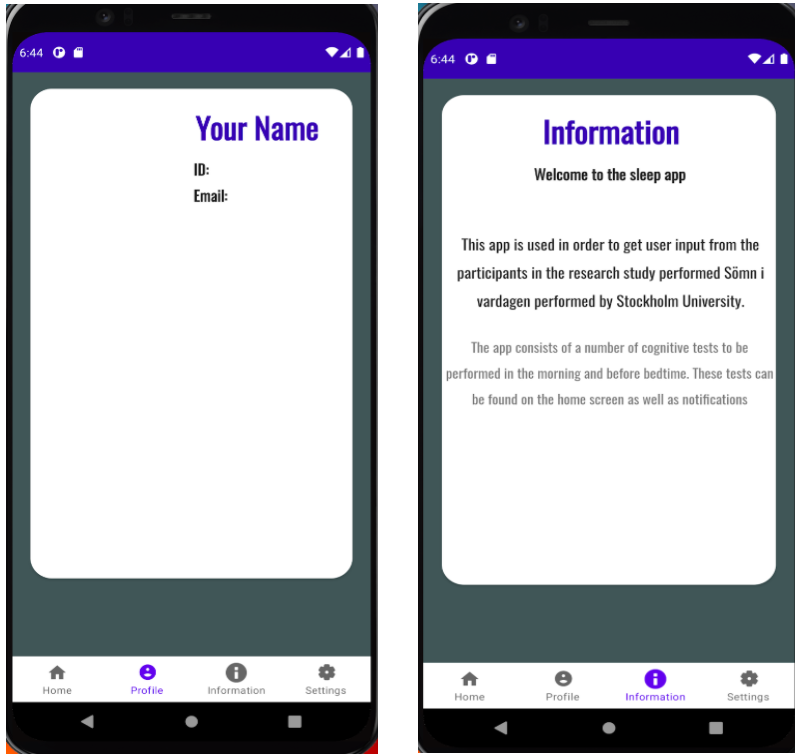
\includegraphics[scale=0.8]{Android3.png}
    \caption{The profile and information screen of the app
}
    \label{fig:android3}
  \end{center}
\end{figure}

\subsubsection{Task Phase}
The task phase was also divided into parts that were developed concurrently, namely the encoding, distraction and recall phases.

\subsubsection{Encoding}
In the encoding phase 9 symbols are displayed in a 3x3 grid, the symbols are pseudo randomly chosen and displayed from a set of icons with the limitation that none of the symbols was presented during the past 5 trials. The user then has 10 seconds to memorize the location of the symbols. For research purposes the symbol location is also saved locally.

\begin{figure}[H]
  \begin{center}
    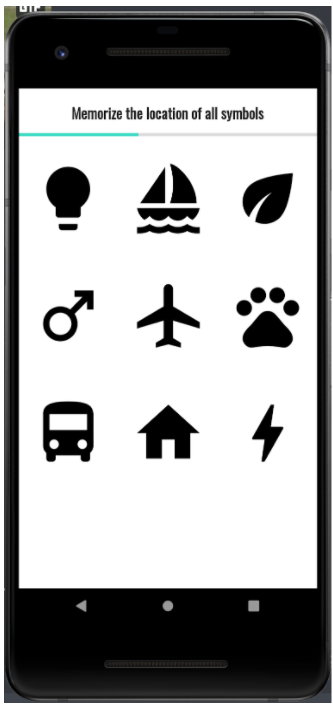
\includegraphics[scale=0.7]{Android4.png}
    \caption{The encoding phase of the task
}
    \label{fig:android4}
  \end{center}
\end{figure}

\subsubsection{Distraction}
In the distraction phase the participant has to touch all F’s as fast as possible
on the 5x9 grid, distribution 30 percent F’s. When a F is pressed it disappears from the grid.

\begin{figure}[!h]
  \begin{center}
    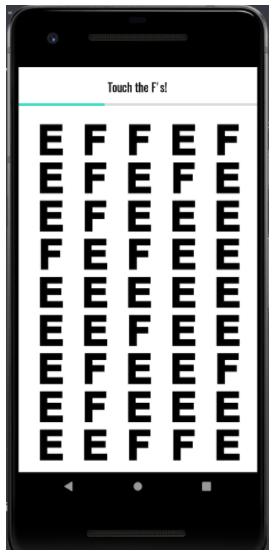
\includegraphics[scale=0.8]{Android5.png}
    \caption{The distraction phase of the task
}
    \label{fig:android5}
  \end{center}
\end{figure}

\subsubsection{Recall}
In the recall phase the participant has to remember the location of one of the symbols from the encoding phase. The participant then has 15 seconds to press it and failure to do so will result in a beeping tone as indication.

\begin{figure}[!h]
  \begin{center}
    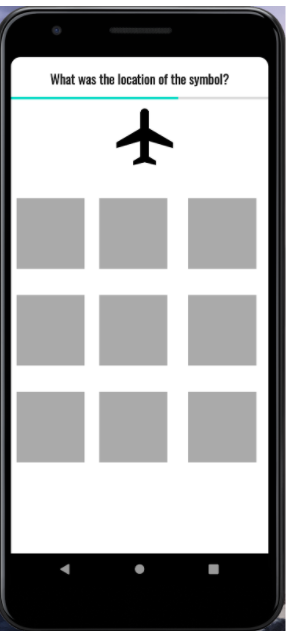
\includegraphics[scale=0.8]{Android6.png}
    \caption{The recall phase of the task
}
    \label{fig:android6}
  \end{center}
\end{figure}


\section{Discussion and analysis}

This chapter includes discussions and analysis of the design process as well as the what impact the final application will have on the market. 

\subsection{Market impact}

The problem that the application developed in this work tries to solve is hugely vital for ensuring good health and happiness amongst people as stated by Dement, W. C., and Vaughan, C in their work “The promise of sleep: A pioneer in sleep medicine explores the vital connection between health, happiness, and a good night's sleep”.\cite{dement_promise_1999} However, the application alone does not bring any solution to this problem, in order for the application to be useful it requires researchers to distribute questionnaires to the users of the application as well as study the collected data together with how the users perform on the cognitive tasks. 

There exists a plethora of different sleep tracking applications in the mobile ecosystem trying to solve the same problem but in different ways which can range from monitoring the users heart rate during the night to help the user establish a good sleep schedule. These applications can often belong to a wider business model in order for the developers to profit. Since the application developed in this work belongs to an academic research study it does not have the requirement of bringing in profits in order to be successful. There do exist similar sleep tracking applications intended for research purposes as for example the STF Sleep Research that is a custom app built for the Stanford Technology Analytics and Genomics in Sleep (STAGES) project to collect actigraph data for research. The app includes a date jiggle feature to ensure data is de-identified as well as the option to collect high resolution data. 
However, the number of sleep trackers intended for scientific research is clearly lower than the number of profit based sleep tracking applications. In addition to this, a sleep application used for research in a scientific study does not have to compete with any other sleep tracking application since the applications used in a particular study is either chosen or completely developed by the researchers performing the study. Regarding the number of substitute products on the market it depends on how one interpret the questions, on one hand it exists a plethora of similar applications on the market, but since our application is specifically designed and developed with the research team’s requirements in mind it can be argued for that does not exist substitute products on the market. 

\subsection{User Experience}

The UX design and implementation is a key component for the user adoption of mobile apps and services and is therefore important to evaluate in projects like this. According to Beyer et.al, innovative design can be a successful driving force for user adoption, however, it should be said that too much innovation can slow down initial user adoption.\cite{beyer_contextual_1998} It’s hard to define innovation and it’s often a subjective matter. But we think that the design of the final application is directed more towards the conservative side of design, which can be a positive thing when developing an application that is going to be used in research where you want to eliminate as many variables as possible in order to be able to draw the correct conclusion about the researched topic.\cite{galitz_essential_2007}

Regarding the usability and intuitiveness of the application the user feedback shows that the application is easy to use, logical and uncomplicated which is the definition of intuitive design.\cite{galitz_essential_2007}
The negative user feedback mainly concerns informational aspects such as the purpose of the distraction phase in the cognitive test, lack of notification before starting the cognitive test and inconsistent use of time estimations.\cite{bevan_usability_1994}' Future work could possibly focus on improving these said things for maximising usability and intuitiveness.  

\subsection{Complexity}

None of the user feedback included comments of the application being complex to use. This is possibly because the number of choices the user can make in the application is limited, contributing to less complexity.\cite{comber_layout_1997} 

\section{Conclusion}

This work has focused on developing mobile applications for use in a research project. One web application was developed with the JQuery framework as well as an Android application. Main focus has been on developing user-friendly interfaces that take usability and intuitiveness into consideration. 
The result is a working web app prototype as well as an integrated Android application, the user feedback shows that the applications are easy to use and intuitive. 

\printbibliography
\end{document}
